%how to cite
%\cite{Seow2011}
%how to add figure
%\ref{fig:TotalConsumption} 

%\begin{figure}[h!]
%	\centering
%	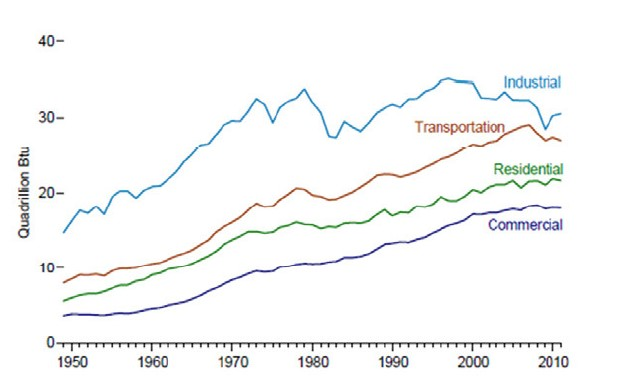
\includegraphics[width=0.8\linewidth]{Figure/Total-consumption.jpg}
%	\caption{Total Consumption by End-Use Sector, 1949-2011 
%   \cite{Apostolos2013}}
%	\label{fig:TotalConsumption}
%\end{figure}



\newpage
\section{Introducci\'on}
\label{chapter1}
%\textit{Person in Charge; }

En el an\'alisis de mercado laboral es posible observar la diversificaci\'on de ocupaciones basadas en la delimitaci\'on geogr\'afica y, en consecuencia, diferentes remuneraciones se generan de acuerdo con el tipo de trabajo. Estas remuneraciones a su vez poseen ciertas diferencias dentro de un mercado competitivo; las mismas se sustentan en la oferta y la demanda de una determinada profesi\'on, e incluso con el nivel de productividad que el capital humano posee. Dada la premisa anterior, cualquier factor que no impacte directamente en el nivel de productividad de un individuo, no deber\'ia afectar a su vez en la remuneraci\'on que el mismo perciba; dicho de otra manera, la religi\'on, color de piel o GENERO no deber\'ian generar diferencias en las remuneraciones. \cite{RodriguezPerez_2014}


A pesar de que en las \'ultimas d\'ecadas las mujeres han aumentado su nivel de educaci\'on y ocupado posiciones laborales de la misma \'indole que los hombres, diferentes organismos han demostrado que existe una gran brecha salaria de g\'enero en el Mundo. Los n\'umeros son tan alarmantes que uno de los objetivos del G-20, es reducir la brecha de genero en un 25\% para el 2025. \cite{G20_2019}

